\documentclass{beamer}
\usetheme{metropolis}
\usepackage{graphicx}
\usepackage{amsmath}
\usepackage{tcolorbox}
\title{Digital Signal Processing: COSC390}
\author{Jordan Hanson}
\institute{Whittier College Department of Physics and Astronomy}

\begin{document}
\maketitle

\begin{frame}{Unit 2.2 Outline}
\begin{enumerate}
\item Types of filters (reading: ch. 3, ch. 5)
\begin{itemize}
\item Butterworth
\item Bessel
\item Chebyshev
\end{itemize}
\item LTI systems and their properties (reading: ch. 5)
\item Convolution (reading: ch. 7)
\begin{itemize}
\item Implementation with FFT
\item Impulse and step response
\end{itemize}
\end{enumerate}
\textbf{These lectures will cover:} (Reading: chapter 19)
\begin{enumerate}
\item \textbf{Common filter kernels: Moving Average}
\item \textbf{General Recursive Filters: HP, LP, and Notch Examples}
\item \textbf{FIR and IIR definitions}
\end{enumerate}
\end{frame}

\section{Common filter kernels: Moving Average}

\begin{frame}{Common filter kernels: Moving Average}
The out of an LTI system such as a filter man be expressed as a \textit{convolution} of the transfer function coefficients $a_k$ and the data $x$. If the output is $y$, we may write
\begin{equation}
y[n] = \sum_{k=0}^{N-1} a_k x[n-k]
\end{equation}
\begin{figure}
\centering
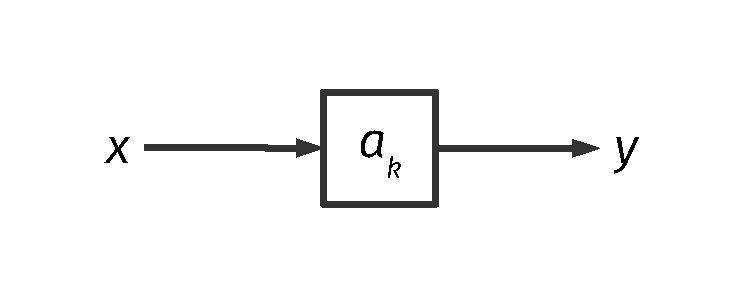
\includegraphics[width=0.6\textwidth]{figures/kernel1.pdf}
\caption{\label{fig:kernel1} A simple model for convolution as an LTI response.}
\end{figure}
\end{frame}

\begin{frame}{Common filter kernels: Moving Average}
The out of an LTI system such as a filter man be expressed as a \textit{convolution} of the transfer function coefficients $a_k$ and the data $x$. If the output is $y$, we may write
\begin{equation}
y[n] = \sum_{k=0}^{N-1} a_k x[n-k] + \sum_{k=0}^{N-1} b_k y[n-k]
\end{equation}
\begin{figure}
\centering
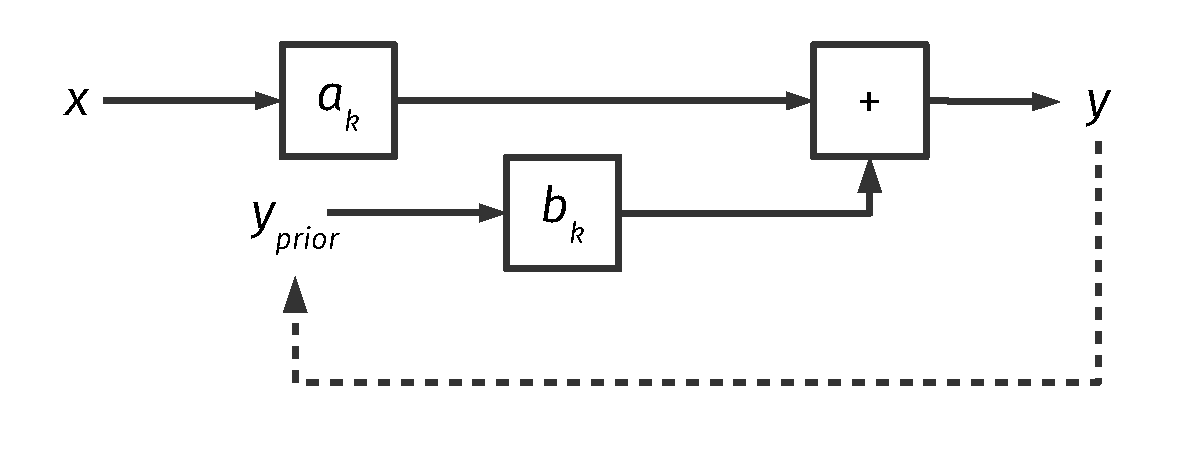
\includegraphics[width=0.75\textwidth]{figures/kernel2.pdf}
\caption{\label{fig:kernel2} A more general model for convolution as an LTI response.  These are the $a$ and $b$ coefficients of the octave \textit{filter} function.}
\end{figure}
\end{frame}

\begin{frame}[fragile]{Common filter kernels: Moving Average}
\textbf{Moving average filter with window-length $n$:}
\begin{enumerate}
\item $a_k$ are all equal to $1/n$
\item $b_k$ are zero
\end{enumerate}
Example:
\begin{itemize}
\item window-3 moving average: $a_0 = \frac{1}{3}$, $a_1 = \frac{1}{3}$, $a_2 = \frac{1}{3}$
\end{itemize}
\begin{verbatim}
y = filter(ones(window,1)/window,1,y);
\end{verbatim}
The filter function is expecting the $a_k$ and $b_k$ coefficients\footnote{For maximum confusion: the textbook and Octave use opposite conventions for $a_k$ and $b_k$.}.
\end{frame}

\section{Octave Programming Exercise: Moving Average}

\begin{frame}[fragile]{Common filter kernels: Moving Average}
Download the code \textbf{movingAverage.m} from Moodle, and run it at your desk.
\begin{enumerate}
\item What is happening to the spectrum?
\item Change the window parameter to various values.  What further changes do you observe in the noise and the spectrum?
\item What function shape do you observe in the spectrum with sufficient window size?
\end{enumerate}
\end{frame}

\begin{frame}{Common filter kernels: Moving Average}
\small
\begin{figure}
\centering
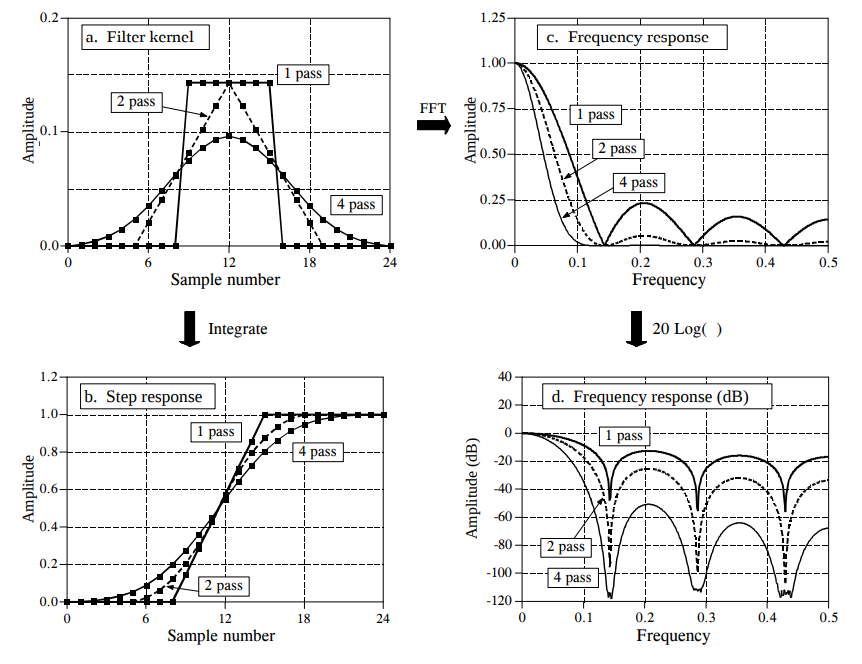
\includegraphics[width=0.7\textwidth]{figures/moving1.png}
\caption{\label{fig:moving1} Various effects of the moving average filter kernel. The moving average efficiently filters high-frequency noise in the time-domain.}
\end{figure}
\end{frame}

\begin{frame}{Common filter kernels: Moving Average}
\small
\begin{figure}
\centering
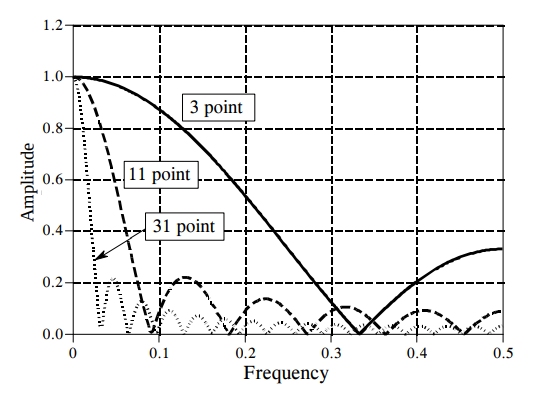
\includegraphics[width=0.7\textwidth]{figures/moving2.png}
\caption{\label{fig:moving2} The frequency response of a moving average filter is a \textit{sync}.  Why? (Calculations on board of filter kernel).}
\end{figure}
\end{frame}

\begin{frame}{Common filter kernels: Moving Average}
Frequency response of moving average filter, n-window:
\begin{equation}
h(f) = \frac{\sin(\pi f n)}{n\sin(\pi f)}
\end{equation}
\begin{itemize}
\item Basically, a sync
\item Modified by n-window instead of period
\end{itemize}
\end{frame}

\begin{frame}{Common filter kernels: Moving Average}
\small
\begin{figure}
\centering
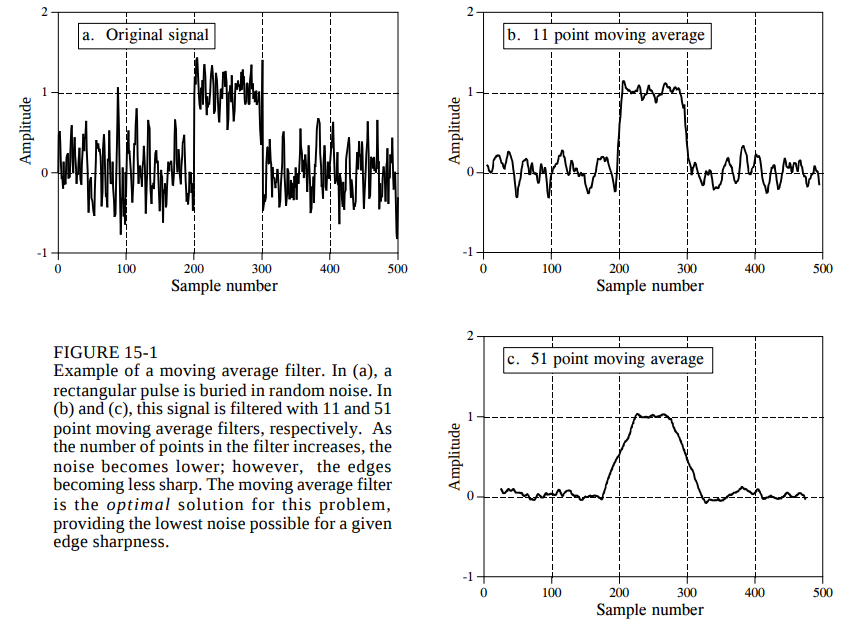
\includegraphics[width=0.7\textwidth]{figures/moving3.png}
\caption{\label{fig:moving3} The moving averege filter removes noise optimally while preserving step response.}
\end{figure}
\end{frame}

\section{Octave Programming Exercise: Finding the Signal}

\begin{frame}[fragile]{Finding the Signal}
Download the code \textbf{movingAverage2.m} from Moodle, and run it at your desk.
\begin{enumerate}
\item By tuning the moving average filter, can you reveal the signal?
\item Bonus: using older code, can you \textit{play this signal as audio} for varying window sizes?
\end{enumerate}
\end{frame}

\section{Octave Programming Exercise: Single-Pole Recursion Formulas}

\begin{frame}[fragile]{Single-Pole Recursion Formulas}
\textbf{Single-pole LP filter recursion:}
\begin{enumerate}
\item $a_0 = 1-x$
\item $b_1 = x$
\end{enumerate}
The variable $x$ varies from $[0,1]$.  It is the amount of decay between samples:
\begin{equation}
x = \exp(-1/d)
\end{equation}
The $x$ parameter is related to the cutoff-frequency:
\begin{equation}
x = \exp(-2\pi f_c)
\end{equation}
\textbf{Exercise:} implement this in movingAverage2.m and recover the signal with the single-pole LP filter.  Note: we are not using the \textbf{butter} function...How would you achieve the effect of multiple poles?
\end{frame}

\begin{frame}[fragile]{Single-Pole Recursion Formulas}
\textbf{Single-pole HP filter recursion:}
\begin{enumerate}
\item $a_0 = (1+x)/2$
\item $a_1 = -(1+x)/2)$
\item $b_1 = x$
\end{enumerate}
The variable $x$ varies from $[0,1]$.  It is the amount of decay between samples:
\begin{equation}
x = \exp(-1/d)
\end{equation}
The $x$ parameter is related to the cutoff-frequency:
\begin{equation}
x = \exp(-2\pi f_c)
\end{equation}
\textbf{Exercise:} implement this in movingAverage2.m and recover the signal with the single-pole HP+LP filter.
\end{frame}

\section{Octave Programming Exercise: Notch and Narrow band-pass}

\begin{frame}[fragile]{Notch and Narrow band-pass}
\small
\textbf{Implement the following recursive formula, and see what it does to noise\footnote{It's probably best to recycle code from movingAverage.m to a new file.}:}
\begin{enumerate}
\item $a_0 = 1-K$
\item $a_1 = 2(K-R)\cos(2\pi f)$
\item $a_2 = R^2-K$
\item $b_1 = 2R\cos(2\pi f)$
\item $b_2 = -R^2$
\end{enumerate}
($R = 1-3 BW$, where $BW$ is the bandwidth, centered on the frequency $f$).  For K, we have
\begin{equation}
K = \frac{1-2R\cos(2\pi f)+R^2}{2-2\cos(2\pi f)}
\end{equation}
\end{frame}

\begin{frame}[fragile]{Notch and Narrow band-pass}
\small
\textbf{Implement the following recursive formula, and see what it does to noise\footnote{It's probably best to recycle code from movingAverage.m to a new file.}:}
\begin{enumerate}
\item $a_0 = K$
\item $a_1 = -2K\cos(2\pi f)$
\item $a_2 = K$
\item $b_1 = 2R\cos(2\pi f)$
\item $b_2 = -R^2$
\end{enumerate}
($R = 1-3 BW$, where $BW$ is the bandwidth, centered on the frequency $f$).
\end{frame}

\begin{frame}[fragile]{Notch and Narrow band-pass}
\begin{enumerate}
\item Add a sine-tone to your noise sample, and then isolate it with the band-pass filter.
\item Now make the noise small, but add several other \textit{unwanted sine-tones} to the data, and filter them out with the band-reject.
\end{enumerate}
So now we start to see how simple it is to clean the data of unwanted noise and signals, using only recursive relationships between input and output data!  However, we must eventually make a distinction between \textbf{FIR and IIR.}
\end{frame}

\begin{frame}[fragile]{FIR and IIR}
FIR - Finite Impulse Response:
\begin{equation}
y[n] = \sum_{k=0}^{N-1} a_k x[n-k]
\end{equation}
IIR - Infinite Impulse Response:
\begin{equation}
y[n] = \sum_{k=0}^{N-1} a_k x[n-k] + \sum_{k=0}^{N-1} b_k y[n-k]
\end{equation}
In the second case, the output power never really drops to zero.
\end{frame}

\section{Theory and Examples: Phase Response}

\begin{frame}{Phase Response}
\small
\begin{figure}
\centering
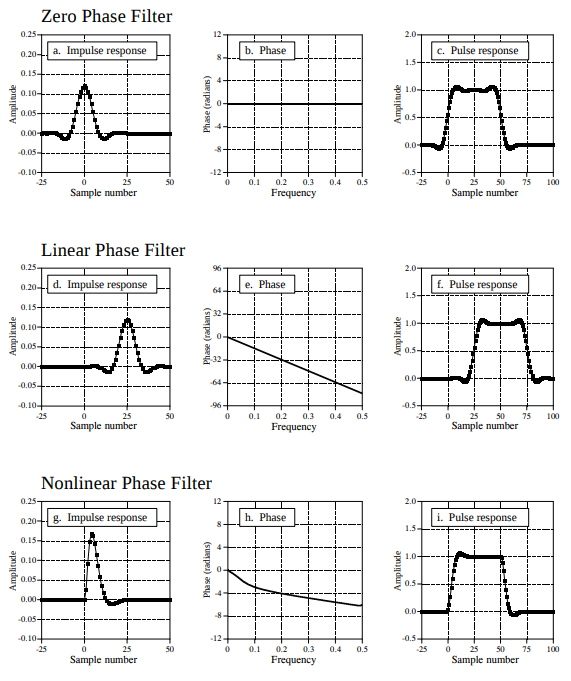
\includegraphics[width=0.5\textwidth]{figures/phase.png}
\caption{\label{fig:phase} The problem with many filters is that they introduce non-zero or non-linear phase response.  How do we eliminate this?}
\end{figure}
\end{frame}

\begin{frame}{Phase Response}
\textbf{Group delay:} reveals dispersion in signals
\begin{equation}
\tau_g = -\frac{d\phi}{d\omega}
\end{equation}
\begin{itemize}
\item What is the Fourier transform of a Gaussian pulse?
\item What is the complex phase of a Gaussian pulse?
\item What is the group delay of the Gaussian pulse?
\end{itemize}
(Observe on board). What if the signal was asymmetric? \textit{Code this in Octave?}
\end{frame}

\section{Aside: Gaussian Fourier Transform}

\begin{frame}{Aside: Gaussian Fourier Transform}
\begin{tcolorbox}[colback=white,colframe=red!40!blue,title=Uncertainty principle for bandwidth]
\alert{The product of the width of a signal in the time domain with the corresponding width in the frequency domain is a constant.
}
\end{tcolorbox}
\end{frame}

\begin{frame}{Phase Response}
\small
\begin{figure}
\centering
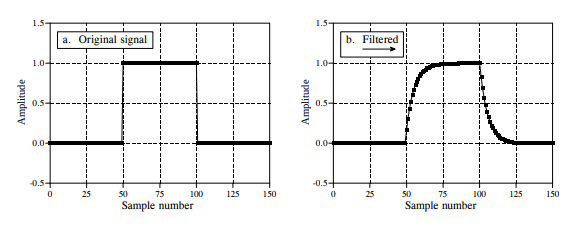
\includegraphics[width=0.75\textwidth]{figures/phase2.png}
\caption{\label{fig:phase2} The effect of the IIR single-pole LP creates a non-linear phase effect.}
\end{figure}
\end{frame}

\begin{frame}{Phase Response}
\small
\begin{figure}
\centering
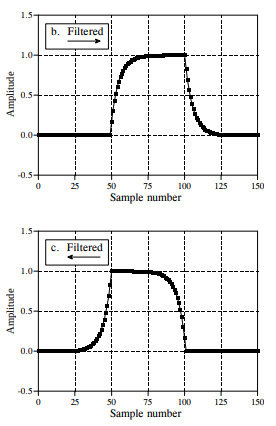
\includegraphics[width=0.33\textwidth]{figures/phase3.png}
\caption{\label{fig:phase3} Reversing the data direction and filtering produces the same power, but a \textit{negative} phase function.}
\end{figure}
\end{frame}

\begin{frame}{Phase Response}
\small
\begin{figure}
\centering
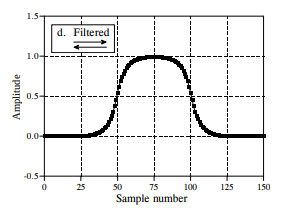
\includegraphics[width=0.5\textwidth]{figures/phase4.png}
\caption{\label{fig:phase4} \textbf{Bi-directional} filtering sets the phase to zero (or linear if there is a time offset).  Group delay should be zero or constant.}
\end{figure}
\end{frame}

\section{Octave Programming Example: Phase Response}

\begin{frame}[fragile]{Octave Programming Example: Phase Response}
Modify either movingAverage.m or FFT.m on Moodle to plot a signal amplitude versus time alongside the phase versus frequency.  Set the noise to zero, and make the signal a Gaussian pulse.
\begin{verbatim}
y = amplitude*exp(-0.5((t-mu).^2/sigma_t^2);
Y = sqrt(conj(fft(y)).*fft(y));
Y_phase = arg(fft(y)); %Phase unwrapping, or...
tan_Y_phase = imag(fft(y))./real(fft(y));
\end{verbatim}
\begin{itemize}
\item Filter twice, flipping the data backwards once, then undo (bi-directional filtering).
\item Now change the data to a square pulse, and repeat.
\end{itemize}
\end{frame}

\section{Correlation}

\begin{frame}{Correlation}
\small
\begin{figure}
\centering
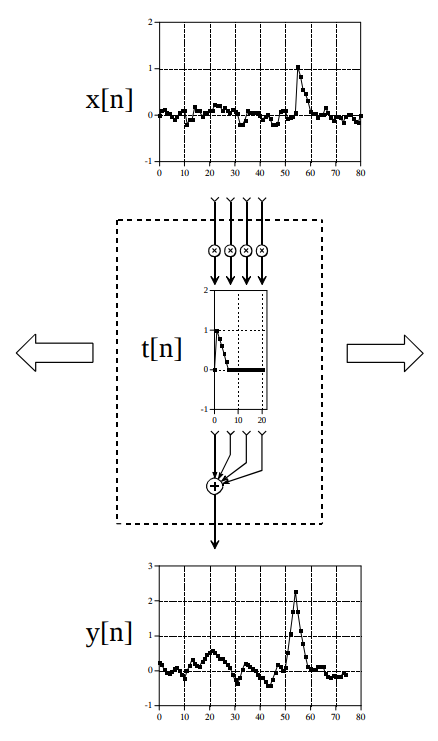
\includegraphics[width=0.3\textwidth]{figures/corr.png}
\caption{\label{fig:corr} Correlation slides a test signal along the data and multiplies them.  The output is summed and is large and positive when the signals align.}
\end{figure}
\end{frame}

\begin{frame}{Correlation}
Correlation between two functions $f$ and $g$:
\begin{equation}
(f * g)(\tau) = \int_{-\infty}^{\infty} f(t)^* g(t+\tau) dt
\end{equation}
Also,
\begin{equation}
F\lbrace f * g \rbrace = F^*(\omega) G(\omega)
\end{equation}
Let's try this in octave by correlating noise+square pulse.
\end{frame}

\section{Conclusion}

\begin{frame}{Unit 2.2 Outline}
\begin{enumerate}
\item Types of filters (reading: ch. 3, ch. 5)
\begin{itemize}
\item Butterworth
\item Bessel
\item Chebyshev
\end{itemize}
\item LTI systems and their properties (reading: ch. 5)
\item Convolution (reading: ch. 7)
\begin{itemize}
\item Implementation with FFT
\item Impulse and step response
\end{itemize}
\end{enumerate}
\textbf{These lectures will cover:} (Reading: chapter 19)
\begin{enumerate}
\item \textbf{Common filter kernels: Moving Average}
\item \textbf{General Recursive Filters: HP, LP, and Notch Examples}
\item \textbf{FIR and IIR definitions}
\end{enumerate}
\end{frame}

\end{document}
